\Subhead{1.1.3}{Параметрическое воздействие на линейные и слабонелинейные колебательные системы}
\textbf{Механизм.} Накачка меняет энергоёмкий параметр, например ёмкость контура. Она умножается на состояние, а не стоит независимой силой справа:
\begin{equation}\label{eq:mathieu}
 \ddot x+2\gamma\dot x+\omega_0^2[1+h\cos\omega_p t]x=0.
\end{equation}
$h$ --- глубина модуляции \emph{квадрата частоты}. Для $C(t)=C_0(1+m\cos\omega_pt)$ имеем $h\simeq-m$; знак меняет фазу, но не порог. В конденсаторе $W=q^2/(2C)$: уменьшение $C$ при большом $|q|$ требует работы привода и повышает энергию; возврат при $q\simeq0$ почти не отбирает её. Максимум $|q|$ бывает дважды за период, отсюда главный резонанс $\omega_p\simeq2\omega_0$. На качелях человек также меняет параметр дважды: поднимает центр масс около нижнего положения, где нагрузка велика, и опускает около крайних положений. Энергия поступает от его работы.

Для $\omega=\omega_p/2$ введём медленные квадратуры. После поворота осей их уравнения можно записать
\begin{equation}
 \dot X=(-\gamma+\kappa)X-\delta Y,\quad
 \dot Y=\delta X+(-\gamma-\kappa)Y,\quad
 \kappa=\frac{|h|\omega_0^2}{4\omega},\quad
 \delta=\frac{\omega_0^2-\omega^2}{2\omega}.
\end{equation}
Их показатели роста $\lambda_\pm=-\gamma\pm\sqrt{\kappa^2-\delta^2}$. Поэтому
\begin{equation}\label{eq:paramthreshold}
 \kappa^2>\gamma^2+\delta^2,\qquad
 |h|_{\rm пор}=\frac{4\gamma}{\omega_0}=\frac2Q
 \quad(\omega_p=2\omega_0).
\end{equation}
И подкачка, и потери пропорциональны энергии: нужен порог их \emph{отношения}, а не минимальная начальная амплитуда. Строго нулевое решение остаётся нулевым; физическую затравку дают флуктуации. Без потерь главная зона $|\omega_p-2\omega_0|<|h|\omega_0/2$; более узкие языки Матье возникают около $2\omega_0/n$.

Линейная модель выше порога даёт экспоненциальный рост. Слабая нелинейность ограничивает его: частотная поправка уводит из резонанса; возможны также нелинейные потери и истощение накачки. Например, для жёсткой кубической поправки $\eta=3\alpha/(8\omega)>0$ стационарная амплитуда $r$ удовлетворяет $\kappa^2=\gamma^2+(\delta+\eta r^2)^2$. На точной настройке физическая ветвь $r^2=\sqrt{\kappa^2-\gamma^2}/\eta$ существует выше порога. Это конкретная модель насыщения, а не универсальный закон любого прибора.
\begin{center}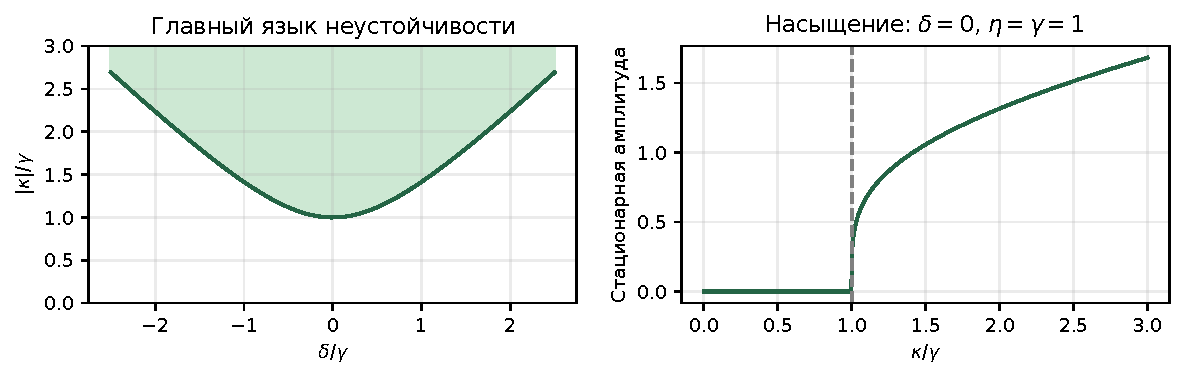
\includegraphics[width=.85\linewidth]{figures/parametric.pdf}\end{center}
% Пятаков, PDF-с.45: гармонический порог 2/Q; с.52: квадратуры.
% На с.45 ступенчатое изменение C даёт иной коэффициент: законы модуляции различны.
